\chapter [Deployment and Results]{Deployment and Results}

\epigraph{"Testing leads to failure, and failure leads to understanding"}{Burt Rutan}

In this chapter is presented the experimental setup used to deploy and test the proposed architecture. First is described the data and hardware and software specifications. Then, two implemented configurations of the system are presented. Finally, results are summarized and analysed.

\section{Experimental Setup}
\todo{First paragraph then figure}
\begin{figure}[ht!]
\centering
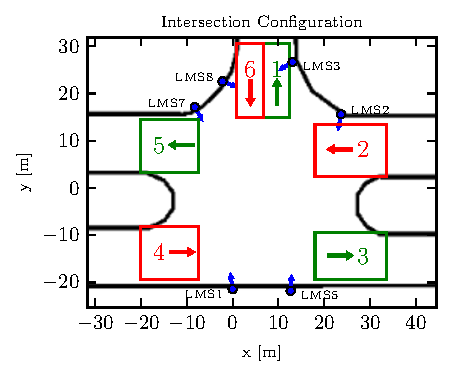
\includegraphics[scale=0.8]{fig/4/intersection-config2.pdf}
\caption{Possi dataset configuration}
\label{possi_img}
\end{figure}

\begin{figure}[ht!]
\centering
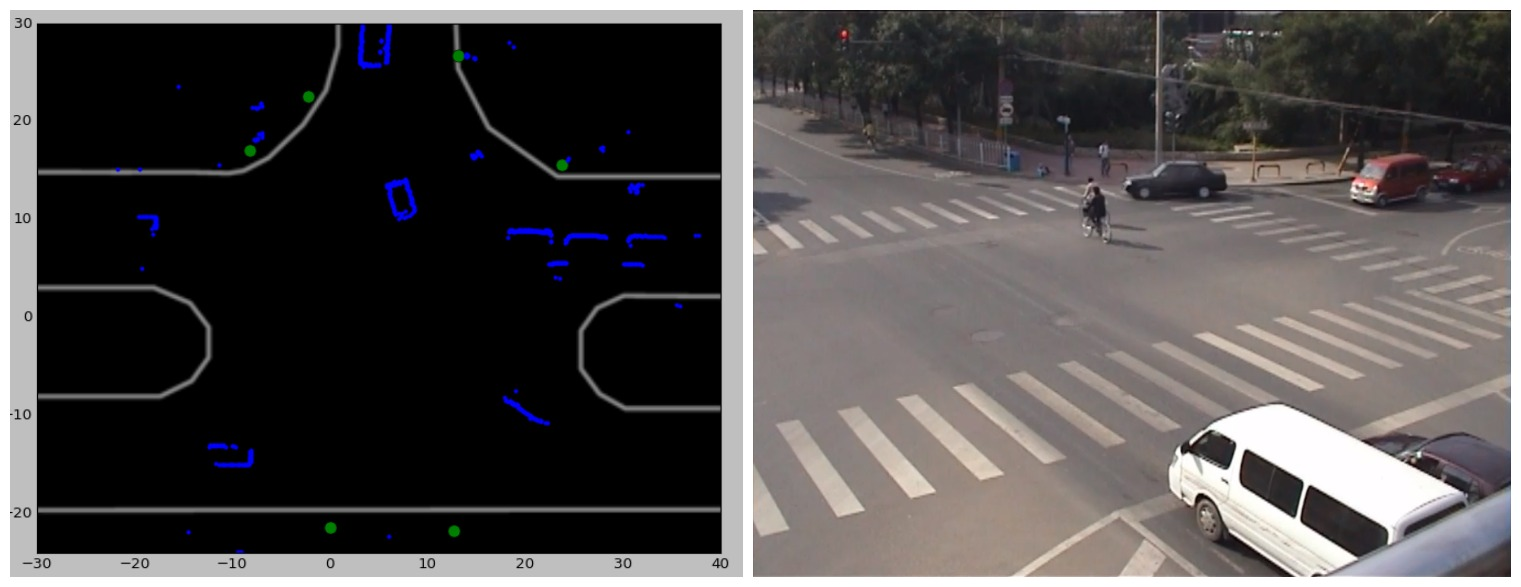
\includegraphics[scale=0.2]{fig/4/sensors_overview.jpeg}
\caption{Overview of sensors data. Left: Laser scanners, Right: Camera.}
\label{possi_sensors}
\end{figure}

%\subsection{Data}
The selected dataset for testing the system is the one from POSSi project (section \ref{possi_ds}). It contains 6 laser-scanners raw readings and a video from a camera located over the intersection. Figure \ref{possi_img} depicts the configuration used by this dataset. In figure \ref{possi_sensors} is shown the data from each type of sensors, laser scanners and camera. The ground truth data used for validation is the vehicle count over 3 of the 5 legs of the intersection, taking into account the time at which a vehicle appears. This groundtruth data was generated manually.

 
%\subsection{Hardware and software specifications}

The platform used for the implementation is a laptop ASUS GL552VW, with 8GB RAM DDR4, a processor Intel Core i7 6700HQ @ 2.60GHz x 8 cores and graphic card Nvidia GeForce GTX 960M. The operating systems running on it is Ubuntu 16.04 LTS. The software was developed using primarily Python3 and C++ as programming languages. Used libraries are MatplotLib, Scikit, Numpy, OpenCV, and darknet for data processing and visualisation. For communication scheme redis was installed along some JSON parsers for formatting.

\section{Test Configurations}
\todo{First paragraph then figure}

\begin{table}[ht!]
\footnotesize
\centering
\begin{tabular}{|c | c| c|}
\hline
\textbf{Proc. Stage} & \textbf{Block ID} & \textbf{Name} \\
\hline

\multirow{2}{*}{Data feeding} &
A & camera\_publisher \\
\cline{2-3} 
& B & laser\_publisher \\
\hline

\multirow{3}{*}{Preprocessing} &
C & laser\_bg\_remover \\
\cline{2-3}
& D & laser\_pol2cart \\
\cline{2-3}
& E & laser\_cart\_merge \\
\hline

\multirow{4}{*}{Feature analysis} &
F & points2clusters \\
\cline{2-3}
& G & points2occgrid \\
\cline{2-3}
& H & camera\_blobs \\
\cline{2-3}
& I & camera\_blobs2occgrid \\
\hline

\multirow{2}{*}{Pattern recognition} &
J & virtual\_sensor\_occupancy \\
\cline{2-3}
& K & virtual\_sensor\_merge \\
\hline

\multirow{2}{*}{Situation Assesment} &
L & virtual\_sensor\_to\_flow\_rate \\
\cline{2-3}
& M & flow\_rate\_to\_flow\_status \\
\hline

\end{tabular}
\caption{Description of processing blocks used in test configurations}
\label{desc_test_config}
\end{table}

In order to test the proposed architecture, two different configurations have been selected. The first configuration is using just the camera information. The second configuration is based on multiple laser sensors along with the camera.

Each configuration consists of a set of processing blocks (as described in section \ref{proc_blocks}) connected, aiming to take data from  lasers and cameras, to produce an output of higher level. In this case, the binary status of a leg (traffic flowing, traffic stopped) is the metric used for evaluation, derived from the vehicle count.

The following table lists all used blocks and assigns an ID for each one. Those IDs are used in the graph description in its own section. Also, bold nodes and connections indicate multiple instance of the same element. The figure \ref{tconf1} shows the  configuration used for processing just video data. Figure \ref{tconf2} shows the configuration when a set of lasers is added to the single-camera configuration. The blue line represents the fusion at node K, which is fusion on virtual sensors level. The purple line represents the fusion at flow rate level.

\todo{Explain evaluation params}

\begin{figure}[ht!]
\centering
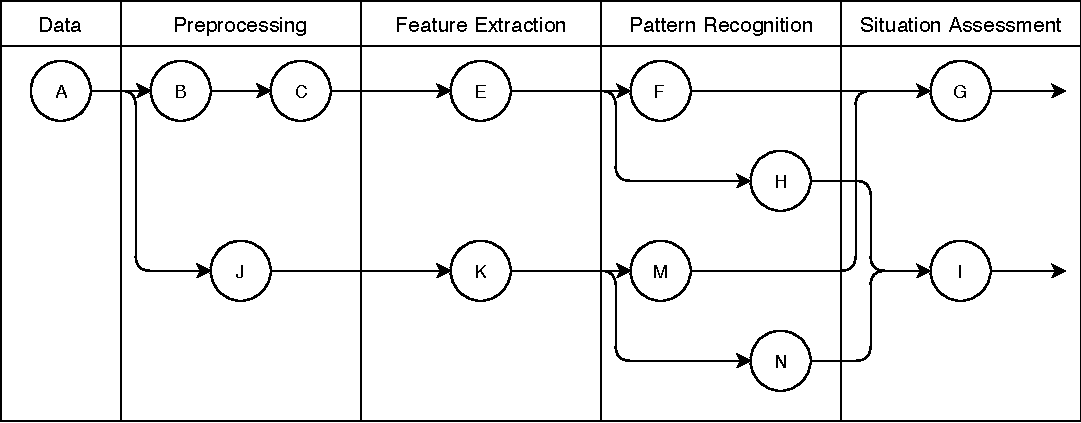
\includegraphics[scale=0.6]{fig/4/test_configuration1.pdf}
\caption{Single camera configuration}
\label{tconf1}
\end{figure}

\begin{figure}[ht!]
\centering
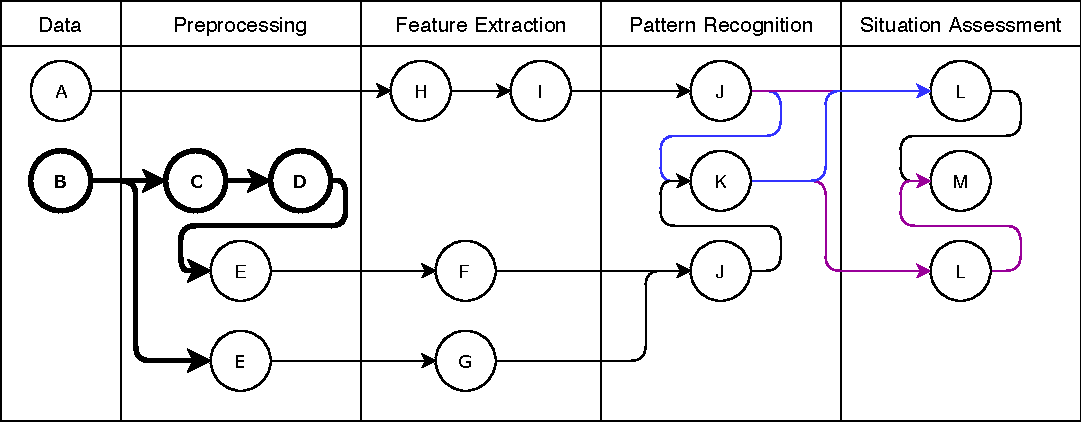
\includegraphics[scale=0.6]{fig/4/test_configuration2.pdf}
\caption{Multiple lasers and camera configuration}
\label{tconf2}
\end{figure}

%TODO

%\subsection{Case 3: Multiple Lasers and camera}
%
%\begin{figure}[ht!]
%\centering
%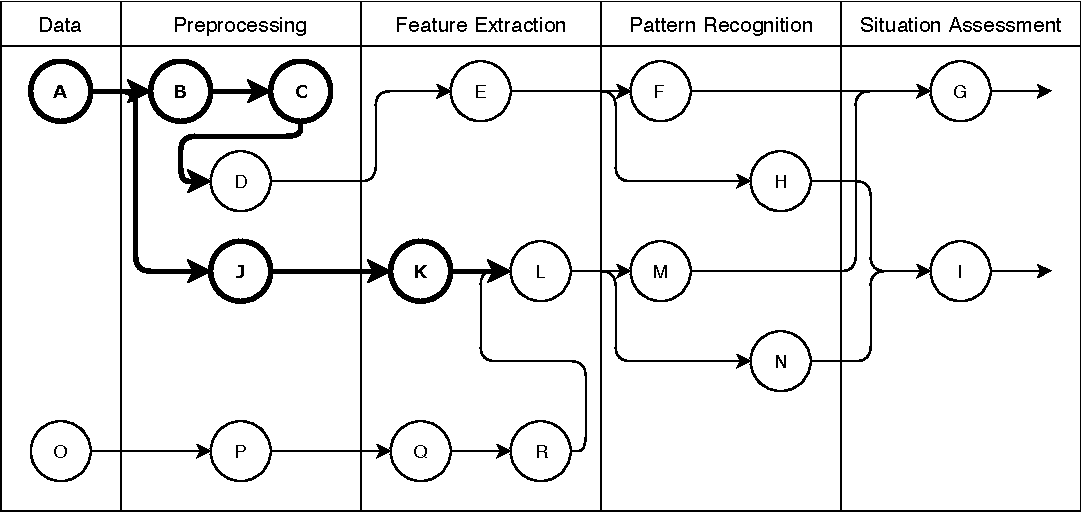
\includegraphics[scale=0.7]{fig/4/test_configuration3.pdf}
%\caption{Multiple lasers and camera configuration}
%\label{tconf3}
%\end{figure}

%TODO

\section{Results}

\subsection{Case 1: Single camera}

As stated before, the flow status is used for comparing the system with the ground truth. This status is derived from the flow rate in vehicles per second. If this value is greater than a defined threshold, it is considerded to be in "traffic flowing" status.

As result of the first stages of processing, vehicle detection in three diferent frames are shown in figure \ref{camera_detection}. This is a representation of the output from node H, camera\_blobs.

\begin{figure}[ht!]
\centering
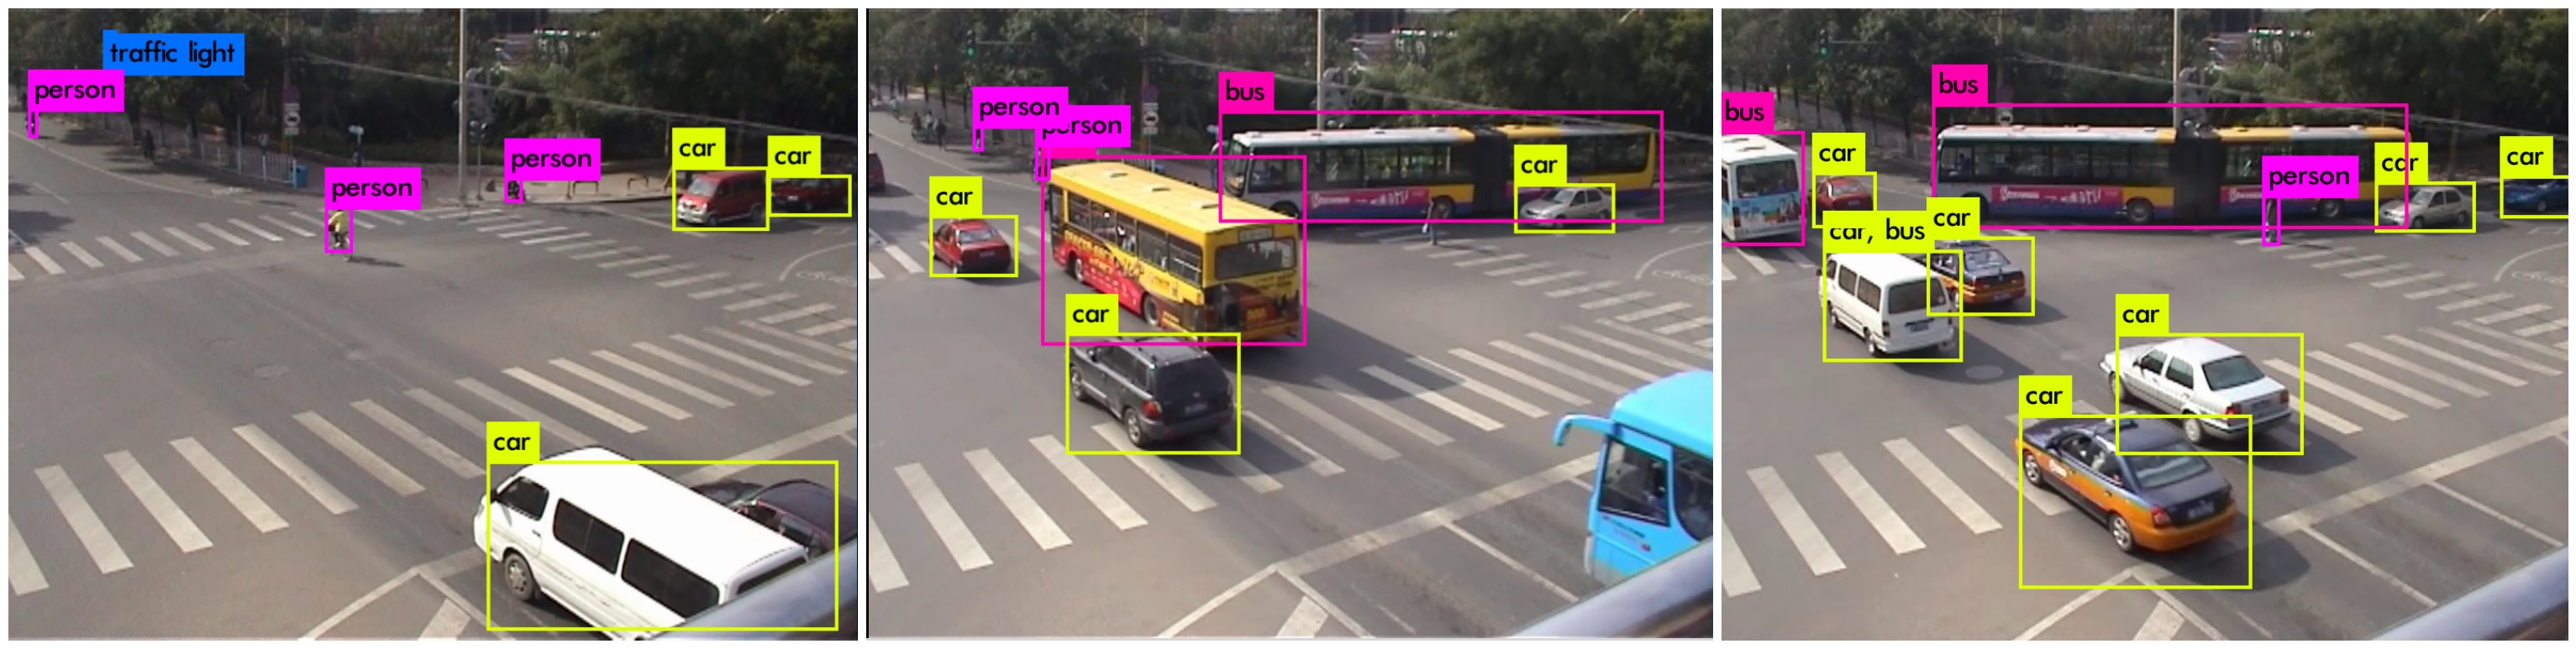
\includegraphics[scale=0.11]{fig/4/camera.jpeg}
\caption{Vehicle detection using camera}
\label{camera_detection}
\end{figure}

In the figure \ref{video_res} is shown the comparison between the flow profile obtained from the system and the generated by the ground truth. There is also remarked one of the intervals where the output is "traffic flowing". After evaluating the performance of the system in a frame basis, a confusion matrix is obtained (table \ref{video_cf}), here $F$ denotes the state "traffic Flowing" and $S$ denotes "traffic Stopped" and we get an accuracy of 91.82\% and a TPR (True Positive Rate) of 55.70\%.

\begin{table}[ht!]
\footnotesize
\centering
\noindent
\renewcommand\arraystretch{1.5}
\setlength\tabcolsep{0pt}
\begin{tabular}{c c c c c}
  \multirow{10}{*}{\rotatebox{90}{\parbox{1.1cm}{\bfseries\centering Actual\\ value}}} & 
    & \multicolumn{2}{c}{\bfseries Outcome} & \\
  & & \bfseries F & \bfseries S & \bfseries total \\
  & F$'$ & \MyBox{694}{} & \MyBox{552}{} & 1246 \\[2.4em]
  & S$'$ & \MyBox{26}{} & \MyBox{5791}{} & 5817 \\
  & total & 720 & 6343 &
\end{tabular}
\caption{Confusion matrix of the system based on video}
\label{video_cf}
\end{table}


\begin{figure}[ht!]
\centering
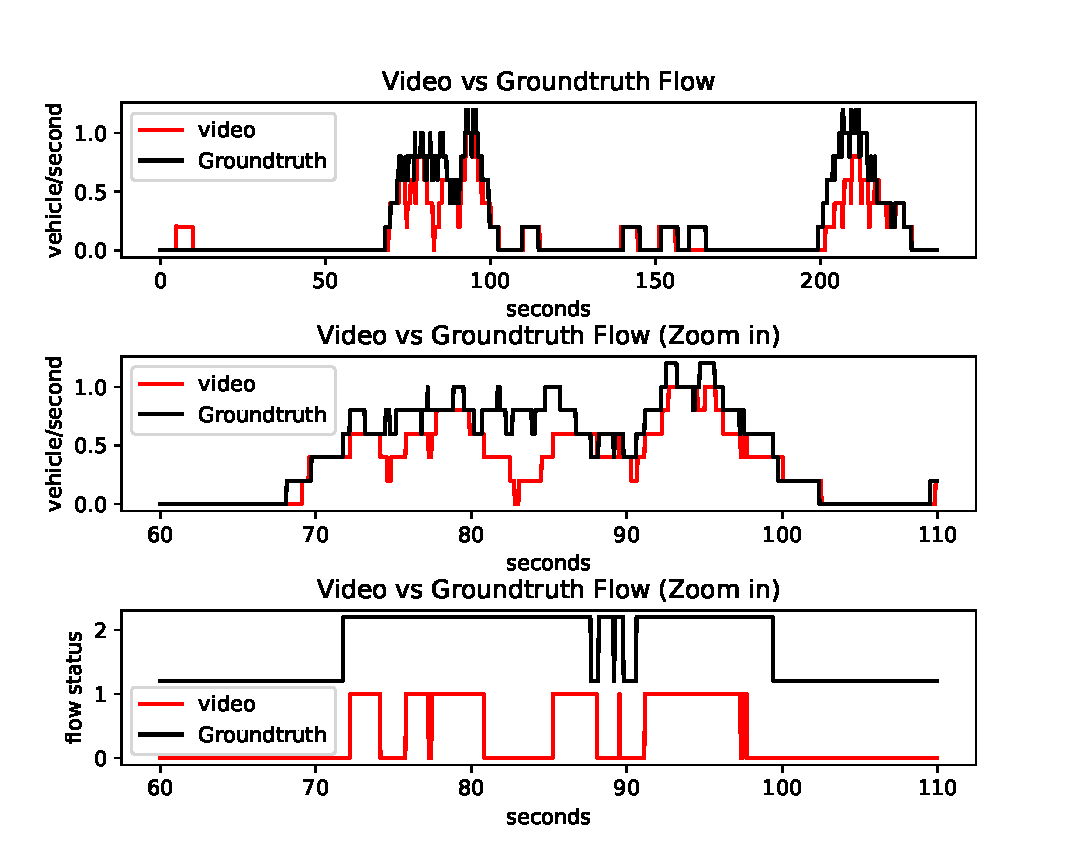
\includegraphics[scale=0.45]{fig/4/video_res.pdf}
\caption{Results for the single camera implementation in one of the legs of the intersection}
\label{video_res}
\end{figure}


\subsection{Case 2: Camera and multiple lasers}
%{'TN': 5791, 'TP': 694, 'FP': 26, 'FN': 552}
%v30 FPR: 0.0045, F1: 0.7060, NPV: 0.5108, reca: 0.5570, spec: 0.9955, PPV: 0.9639, accu: 0.9182, prec: 0.9639, TPR: 0.5570, prev: 0.1764, 
%{'TN': 5650, 'TP': 23, 'FP': 167, 'FN': 1223}
%l30 FPR: 0.0287, F1: 0.0320, NPV: 0.0156, reca: 0.0185, spec: 0.9713, PPV: 0.1211, accu: 0.8032, prec: 0.1211, TPR: 0.0185, prev: 0.1764, 
%{'TN': 5414, 'TP': 1098, 'FP': 403, 'FN': 148}
%vl_avg_1_30 FPR: 0.0693, F1: 0.7994, NPV: 0.9216, reca: 0.8812, spec: 0.9307, PPV: 0.7315, accu: 0.9220, prec: 0.7315, TPR: 0.8812, prev: 0.1764, 
%{'TN': 5669, 'TP': 792, 'FP': 148, 'FN': 454}
%vl_max_1_30 FPR: 0.0254, F1: 0.7246, NPV: 0.6039, reca: 0.6356, spec: 0.9746, PPV: 0.8426, accu: 0.9148, prec: 0.8426, TPR: 0.6356, prev: 0.1764, 
%{'TN': 5804, 'TP': 161, 'FP': 13, 'FN': 1085}
%vl_f_avg_30 FPR: 0.0022, F1: 0.2268, NPV: 0.1091, reca: 0.1292, spec: 0.9978, PPV: 0.9253, accu: 0.8445, prec: 0.9253, TPR: 0.1292, prev: 0.1764, 
%{'TN': 5624, 'TP': 716, 'FP': 193, 'FN': 530}
%vl_f_max_30 FPR: 0.0332, F1: 0.6645, NPV: 0.5432, reca: 0.5746, spec: 0.9668, PPV: 0.7877, accu: 0.8976, prec: 0.7877, TPR: 0.5746, prev: 0.1764,

%v30         reca: 0.5570, spec: 0.9955, accu: 0.9182, prec: 0.9639, TPR: 0.5570,
%vl_avg_1_30 reca: 0.8812, spec: 0.9307, accu: 0.9220, prec: 0.7315, TPR: 0.8812,
%vl_max_1_30 reca: 0.6356, spec: 0.9746, accu: 0.9148, prec: 0.8426, TPR: 0.6356,
%vl_f_avg_30 reca: 0.1292, spec: 0.9978, accu: 0.8445, prec: 0.9253, TPR: 0.1292,
%vl_f_max_30 reca: 0.5746, spec: 0.9668, accu: 0.8976, prec: 0.7877, TPR: 0.5746

In this test case, the information from the laser scanners is used with the purpose of increase the performance of the system. This required just to include the appropiate nodes for laser data processing, and replace some nodes from the video processing graph to allow data fusion from laser and cameras. An example of vehicle detection based on laser scanners is shown in figure \ref{laser_detection}. This is the output of the node F, points2clusters.

\begin{figure}[htb!]
\centering
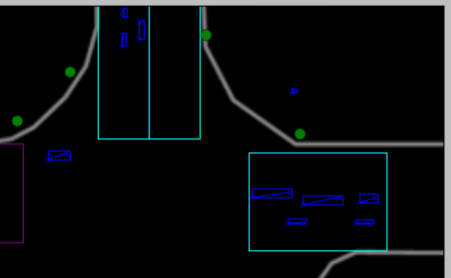
\includegraphics[scale=0.4]{fig/4/laser1a.png}
\caption{Vehicle detection using laser scanners}
\label{laser_detection}
\end{figure}

For merging information from laser and cameras, it was decided to perform the fusion at two levels, at the virtual sensor occupancy level and at the flow rate level. Both of these approaches were implemented using average and maximum policies. In the figure \ref{vl_res} is depicted the flow rate output for all of four configurations.

Performing the same frame-based analysis as for the video system, we obtain the confusion matrices presented in table \ref{vl_cf}. It is noted that performing the fusion at virtual sensor occupancy level, the accuracy of the systems has almost no change, 92.2\% and 91.48\% for average and maximum policies respectively. For the TPR, there is a significative increase, having 88.12\% and 63.56\%, also for average and maximum policies.

When the fusion is performed at flow rate level using average policy, the accuracy and TPR values are reduced to 84.45\% and 12.92\%. Using maximum policy, there is a small decrement in the values, with an accuracy of 89.76\% and a TPR of 57.46\%.

\begin{figure}[htb!]
\centering
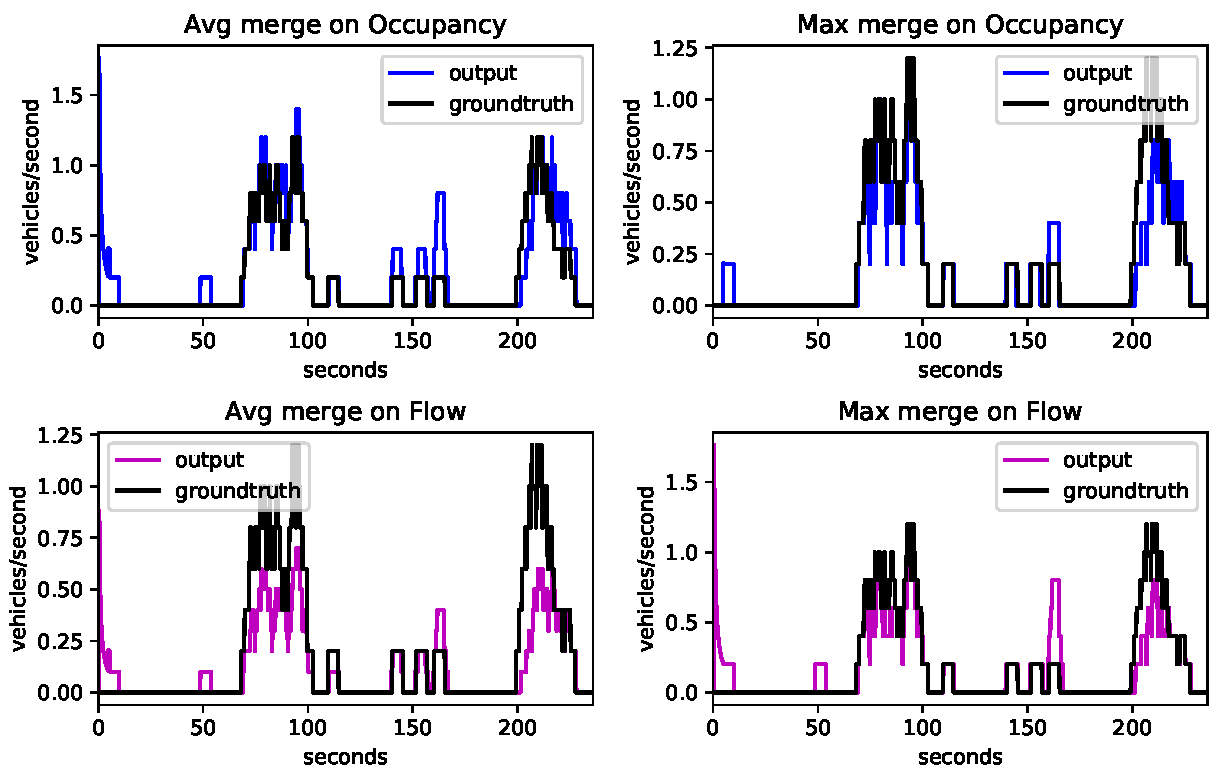
\includegraphics[scale=0.5]{fig/4/vl_res.pdf}
\caption{Results for the multisensor implementation using four different fusion approaches}
\label{vl_res}
\end{figure}

\begin{table}[htb!]
\footnotesize
\centering
\noindent
\renewcommand\arraystretch{1.5}
\setlength\tabcolsep{0pt}
\begin{tabular}{c c c c c}
  \multirow{10}{*}{\rotatebox{90}{\parbox{1.1cm}{\bfseries\centering Actual\\ value}}} & 
     \multicolumn{4}{c}{\bfseries Outcome (avg vs\_occ)} \\
  & & \bfseries F & \bfseries S & \bfseries total \\
  & F$'$ & \MyBox{1098}{} & \MyBox{148}{} & 1246 \\[2.4em]
  & S$'$ & \MyBox{403}{} & \MyBox{5414}{} & 5817 \\
  & total & 1501 & 5562 &
\end{tabular}

\begin{tabular}{c c c c c}
  \multirow{10}{*}{\rotatebox{90}{\parbox{1.1cm}{\bfseries\centering Actual\\ value}}} & 
     \multicolumn{4}{c}{\bfseries Outcome (max vs\_occ)}  \\
  & & \bfseries F & \bfseries S & \bfseries total \\
  & F$'$ & \MyBox{792}{} & \MyBox{454}{} & 1246 \\[2.4em]
  & S$'$ & \MyBox{148}{} & \MyBox{5669}{} & 5817 \\
  & total & 940 & 6123 &
\end{tabular}

\begin{tabular}{c c c c c}
  \multirow{10}{*}{\rotatebox{90}{\parbox{1.1cm}{\bfseries\centering Actual\\ value}}} & 
     \multicolumn{4}{c}{\bfseries Outcome (avg flow)} \\
  & & \bfseries F & \bfseries S & \bfseries total \\
  & F$'$ & \MyBox{161}{} & \MyBox{1085}{} & 1246 \\[2.4em]
  & S$'$ & \MyBox{13}{} & \MyBox{5804}{} & 5817 \\
  & total & 174 & 6889 &
\end{tabular}

\begin{tabular}{c c c c c}
  \multirow{10}{*}{\rotatebox{90}{\parbox{1.1cm}{\bfseries\centering Actual\\ value}}} & 
     \multicolumn{4}{c}{\bfseries Outcome (max flow)}  \\
  & & \bfseries F & \bfseries S & \bfseries total \\
  & F$'$ & \MyBox{716}{} & \MyBox{530}{} & 1246 \\[2.4em]
  & S$'$ & \MyBox{193}{} & \MyBox{5624}{} & 5817 \\
  & total & 909 & 6154 &
\end{tabular}

\caption{Fusion configurations from top to bottom: Average on virtual sensor occupancy, Maximum on virtual sensor occupancy, Average on flow rate, Maximum on flow rate}
\label{vl_cf}
\end{table}

\section{Conclusions}

\todo{Sumarise and discuss results}

An intersection management system is a complex set of subsystems, and for a feasible implementation and deployment as a real solution it is needed for it to be easily tested, adapted and enhanced. In this case, after having a well-concieved block design, it was relatively straight forward to start building a video based system for getting an indicator about traffic flow in an intersection using a dataset.

For stakeholders of the system outcome, high level indicators are desired, like traffic status, no matter which low-level hardware or software are used. For this reason, modularity and definitions on data and messages types, allow development of new features without compromising the integrity of the system. Also, new sources of information and data could be easily integrated if the processing of them is made according to the definitions. In that way, it was possible to integrate laser scanner data provided by the dataset, taking into account to generate outputs already defined by the messages specification.

For different sources of information it is not enough to perform a fusion strategy to obtain better results. It is needed to analyse the type of data and the level at which fusion should be performed. Also, it is important to understand if the fusion is competitive, complementary or cooperative, in order to select the appropiate strategy and increase the performance of the system. An example of this, was found when fusing data from camera and lasers at two different levels and using different strategies. It was clear from the results that altough the data was the same, one configuration increased the performace while another one decrease it.





